\section{Validation}

We developed a web service choreography to be our test bed for getting information and developing the Rehearsal Framework. Thus, we will use this choreography to collect information about how we are going to verify its scalability. In this chapter, we will explain how it works.

The choreography implements a service of a supermarket of the future. Based on a list of supermarkets, we are able to get the lowest price possible of a desired product list. For each product, the choreography gets it from the supermarket that offers it with the lowest price. Therefore, we will purchase a list of products with the lowest price possible from a list of supermarkets.

\subsection{Participants of the choreography}
\label{participantschoreography}

The choreography has five participants. Their roles and API are described bellow:
\begin{description}
\item[SMRegistry] The SMRegistry service stores a list of services that implements the supermarket role. Its methods are presented on Table \ref{smregistryapi}.
	\begin{table}[htdp]
	\caption{SMRegistry API}
	\begin{center}
	\begin{tabular}{|c|c|c|m{4cm}|}
		\hline
		Method & Input & Output & Description \\ \hline
		addSupermarket & endpoint : String & confirmation : String & Add a new supermarket endpoint to the supermarket list \\ \hline
		getList & & supermarkets: List<String> & Return a list of supermarket endpoints \\ \hline
	\end{tabular}
	\end{center}
	\label{smregistryapi}
	\end{table}%

\item[SupermarketRole] The choreography can have multiple supermarkets, each supermarket must implement the Supermarket Role API, presented on Table \ref{smroleapi}. It must return the price of a product, and purchase a list of products.
	\begin{table}[htdp]
	\caption{Supermarket Role API}
	\begin{center}
	\begin{tabular}{|c|m{3.5cm}|m{3.5cm}|m{4cm}|}
		\hline
		Method				& Input						& Output 					& Description \\ \hline
		searchForProduct 		& name: String					& name: String, price: Double 	& Get the product price of this supermarket \\ \hline
		registerSupermarket		& endpoint: String				& confirmation: String		& Register the Supermarket endpoint in the RegistrySM service \\ \hline
		purchase				& id: String, personalDataType: data & confirmation: String		& Make the purchase with the order ID and the user address \\ \hline
	\end{tabular}
	\end{center}
	\label{smroleapi}
	\end{table}%
	
\item[Customer] The Customer service is the interface of the choreography. The user can communicates with the other service separately, however the complete functionalities of the choreography is accessible by this service. Its implementation is an orchestration that communicates with the SMRegistry service to get the list of Supermarket services registered and communicates with all of them to get the minimum price possible of the product list. After returning the order, the user can communicates with the Customer to request a purchase and the delivery informations. Its API is presented on Table \ref{customerapi}.
	\begin{table}[htdp]
	\caption{Customer API}
	\begin{center}
	\begin{tabular}{|c|m{3.5cm}|m{3.5cm}|m{4cm}|}
		\hline
		Method				& Input					& Output 					& Description \\ \hline
		getPriceOfProductList	& products: List<String> & order: Order & Return the minimum price of a product list and the id of the order\\ \hline
		purchase 				& id: String, account: accountType & shipper: String & Make the purchase of the products requested with the operation above \\ \hline
		getDeliveryData 		& shipper: String, orderID: String & delivery: String & Get information about the delivery of an order \\ \hline
		
	\end{tabular}
	\end{center}
	\label{customerapi}
	\end{table}%

\item[Shipper] The Shipper service is responsible to stores information about the delivery of products to an address. The shipper receives information about an order from a Supermarket service and send delivery information of an order to the Custumer Service. Table \ref{shipperapi} shows its API.

	\begin{table}[htdp]
	\caption{Shipper API}
	\begin{center}
		\begin{tabular}{|c|c|c|m{4cm}|}
		\hline
		Method			& Input					& Output 					& Description \\ \hline
		setDelivery		& id: String, zipcode: String	& confirmation: String		& Receives the zipcode of an order \\ \hline
		getDataAndTime	& id: String				& time: String				& Returns the time that the order will be delivered \\ \hline
	\end{tabular}
	\end{center}
	\label{shipperapi}
	\end{table}%
	\end{description}
	
\subsection{The workflow}
The choreography has three operations as described in the participant Customer of Subsection \ref{participantschoreography}. Before purchasing an list of products, the user must send this list to the Customer to book them and verify the price. After that, the user can purchase them providing the \emph{id} of the order. Finally, its possible to verify the delivery status to know when the product will arrive. Another message flow that does not happen with these operations is the registering of a Supermarket service in the RegistrySM service. Figure \ref{futuremartConversation} describes a global view of the conversation between the services using BPMN2\footnote{http://www.bpmn.org}.

\begin{figure}[htbp]
\begin{center}
	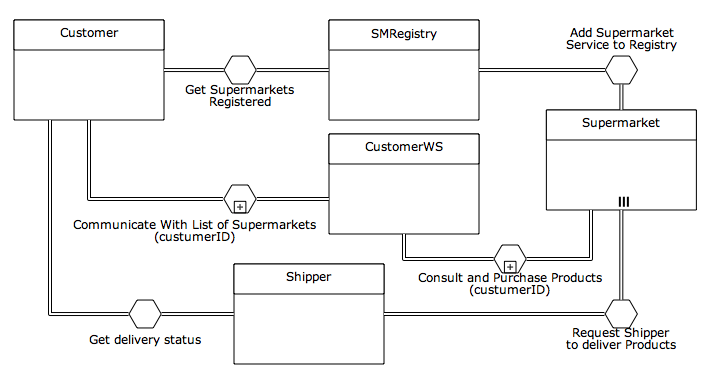
\includegraphics[width=\textwidth]{images/futuremartConversation}
\caption{Global conversation between the services of the Futuremart Choreography}
\label{futuremartConversation}
\end{center}
\end{figure}

\subsubsection{The \emph{getPriceOfProductList} workflow}
Figure \ref{getPriceOfProductListworkflow} shows a BPMN Collaboration diagram of the getPriceOfProductList operation. Each lane represents a participant of the choreography. The getPriceOfProductList operation starts with the Customer participant receiving a request with a list of products. It requests to the SMRegistry participant a list of Supermarket services registered. The registry service collects, from its database, all service endpoints stored and returns it to the Customer.

The Customer stores this list and the product list in its database. Then, it calculates the minimum price possible. The process, that calculates the price, request, for each product,  the product price to all Supermarket.  

The Supermarket lane represents all Supermarket services, the three little vertical lines inside it symbolizes a multiplicity of participants. When each of them receives a request, it verifies in its database what is the price for the specific product to return to the Customer. If the price received is lower then the current lowest, it stores it with the endpoint of the Supermarket service that offer it. 

After checking out and storing all the products price with their respective supermarkets, the Customer returns the price and an id that represents this order.

\begin{figure}[htbp]
\begin{center}
	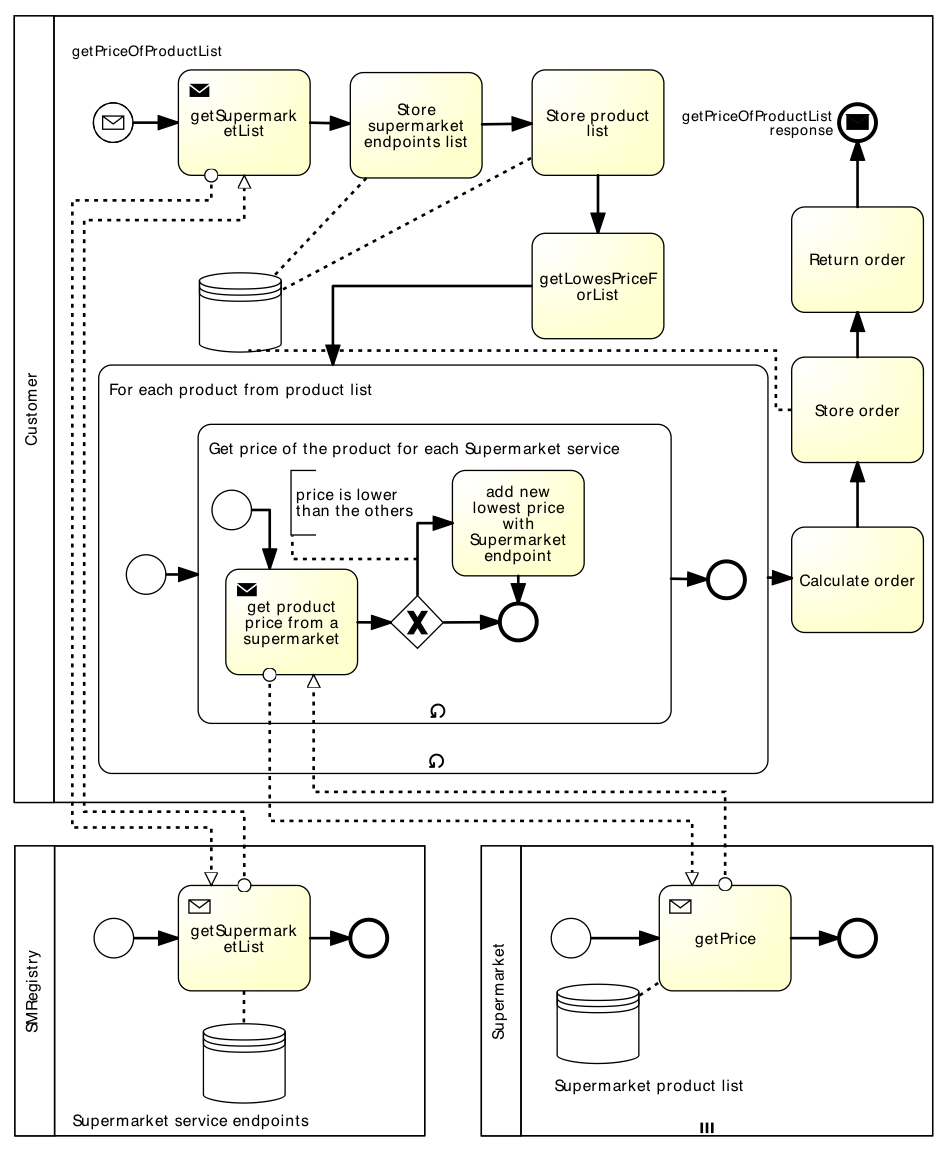
\includegraphics{images/getPriceOfProductListworkflow}
\caption{BPMN Collaboration diagram of the choreography operation \emph{getPriceOfProductList}}
\label{getPriceOfProductListworkflow}
\end{center}
\end{figure}

\subsubsection{The \emph{purchase} workflow}
After ordering a list of products and getting the best price for it, the user can request the purchase. The Customer service receives the request with the order ID and the address of the user. Subsequently, starts a loop that purchases the products related to each Supermarket service.

When a Supermarket service receives a purchase request, it sends a message to the Shipper service to deliver the products. After that, it returns a message to the Customer with the Shipper service endpoint that will deliver the products.

The Shipper service stores the delivery information in its database for future verifications. Finally, the Customer service returns to the user a confirmation with the Shipper service endpoint that will deliver the products. Figure \ref{purchaseworkflow} describes the collaboration between the services that participates in this functionality.

\begin{figure}[htbp]
\begin{center}
	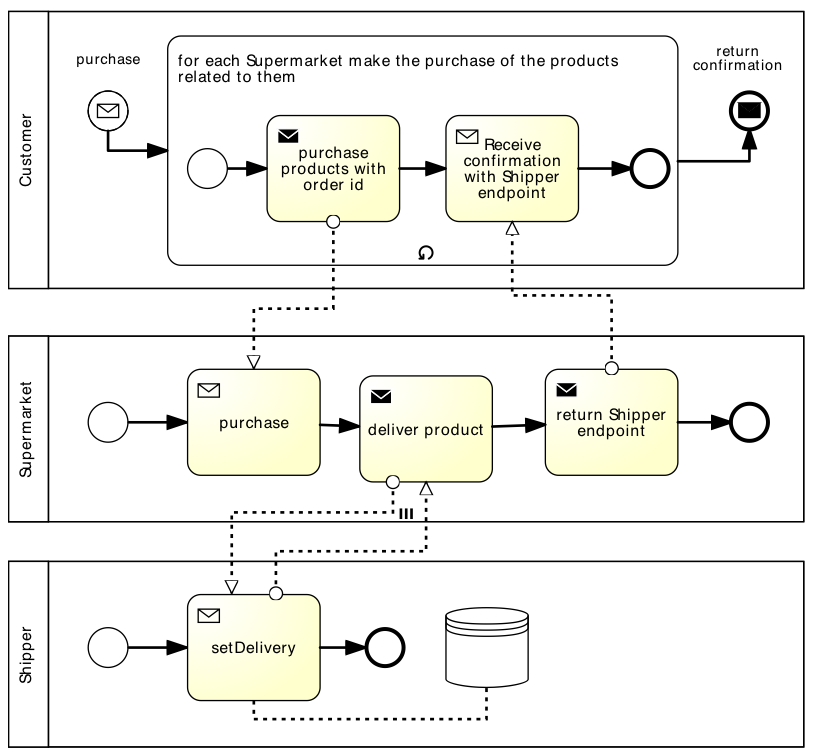
\includegraphics{images/purchaseworkflow}
\caption{BPMN Collaboration diagram of the choreography operation \emph{purchase}}
\label{purchaseworkflow}
\end{center}
\end{figure}

\subsubsection{The \emph{getDeliveryData} workflow}
The user can also verify the delivery status of an order. The Customer service has the getDeliveryData operation that receives an order ID and the Shipper service endpoint. It sends a message to the Shipper requesting the status of an order. The latter collects from its database the order information and returns it. As we can see in Figure \ref{getDeliveryDataworkflow}, the Customer simply returns this data to the user.

\begin{figure}[htbp]
\begin{center}
	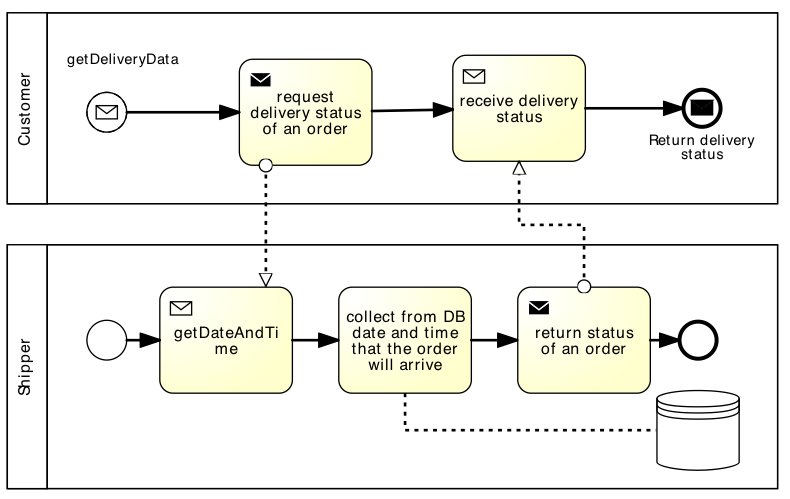
\includegraphics{images/getDeliveryDataworkflow}
\caption{BPMN Collaboration diagram of the choreography operation \emph{getDeliveryData}}
\label{getDeliveryDataworkflow}
\end{center}
\end{figure}

\subsubsection{The \emph{registerSupermarket} workflow}
The registerSupermarket operation is not for the final user of the choreography, but for the user that administrates a Supermarket service. A service that implements the Supermarket role, can register itself into the RegistrySM service, that has a list of all Supermarket services. Figure \ref{registerSupermarketworkflow} describes this registration. A Supermarket service sends a message to register itself. The registrySM service receives this request and stores the service endpoint in its database and returns a confirmation.

\begin{figure}[htbp]
\begin{center}
	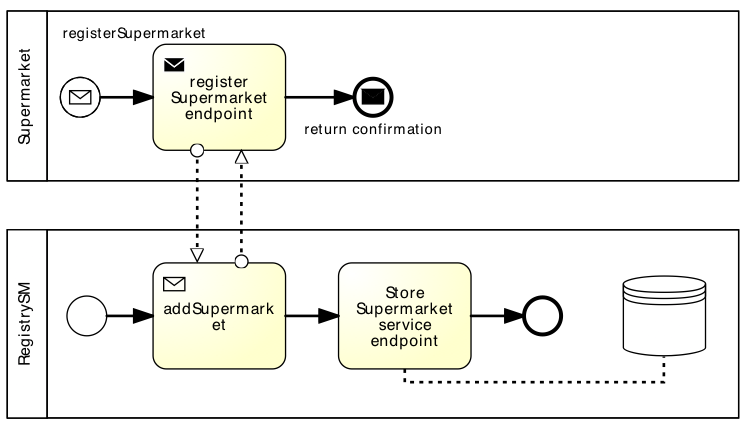
\includegraphics{images/registerSupermarketworkflow}
\caption{BPMN Collaboration diagram of the choreography operation \emph{registerSupermarket}}
\label{registerSupermarketworkflow}
\end{center}
\end{figure}

\subsection{Testing the choreography}

